
%mainfile: Population_growth_model.tex

\pagestyle{fancy} 
\lhead{Atelier Nueromodélisation, 2017}
\rhead{Problem set \#1}
\rfoot{\thepage}
\cfoot{}
\lfoot{~\theauthor}
\renewcommand{\headrulewidth}{0.4pt}
\renewcommand{\footrulewidth}{0.4pt}

\title{Problem Set \#1: Population Growth Model \vspace{-0.5em}}
%\preauthor{} \postauthor{} 
\author{Hsieh Yu-Guan}
\selectlanguage{USenglish}
\date{\formatdate{10}{3}{2017}}
%\date{\today}
\maketitle

\thispagestyle{fancy}

\section{Problem description}

Here we want to model the growth of an animal population. Every year, 
the growth of the population is determined according to its original size.
The population value of each year that we get will be stored in an array 
$p$ so that we can plot its evolution over time.

\section{When growth rate $\alpha$ stays constant}

As a first approximation, we suppose that the growth rate $\alpha$ is contant.
That is, for all $n$, we can write $p_n = p_{n-1} + \alpha p_{n-1}$, where 
$p_n$ is the population value of the $n^{th}$ year (counting from zero) and 
$\alpha$ doesn't depend on $n$.

At first, we fix $p_0 = 2$ and $\alpha = 0.1$ and simulate the population 
growth over a hundred years. The result is shown below:

\vspace{-1em}
\begin{figure}[H]
  \centering
  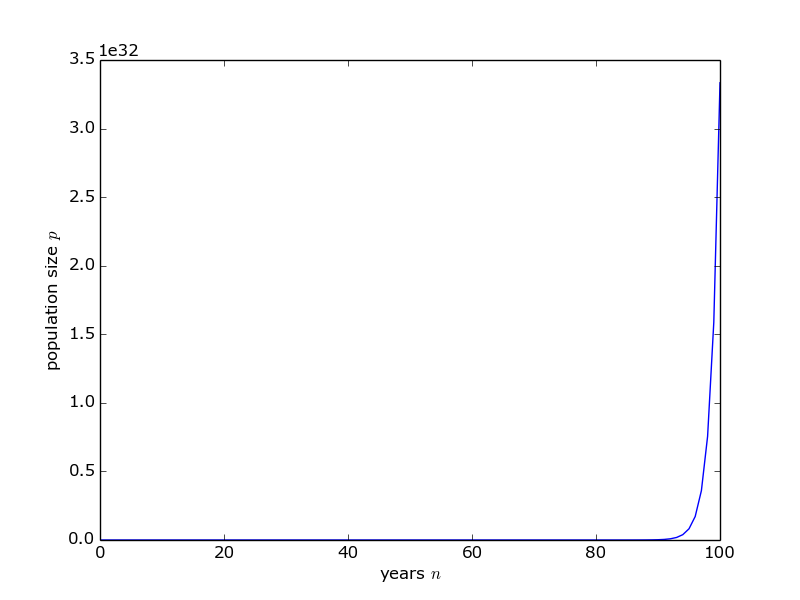
\includegraphics[width=0.7\linewidth]{fig1}
  \caption{Population growth with $p_0 = 2$ and $\alpha = 0.1$}
\end{figure}

As we can see, the population grows exponentially and explodes very fast, 
$10^{32}$ individuals at the end of a century! But it's somehow not very 
surprising because it's exactly what our equation indicates as it can also
be written in the form $p_n = (1+\alpha)p_{n-1}$. Now let's change the value 
of $\alpha$ and see what happens.

\vspace{-1em}
\begin{figure}[H]
  \centering
  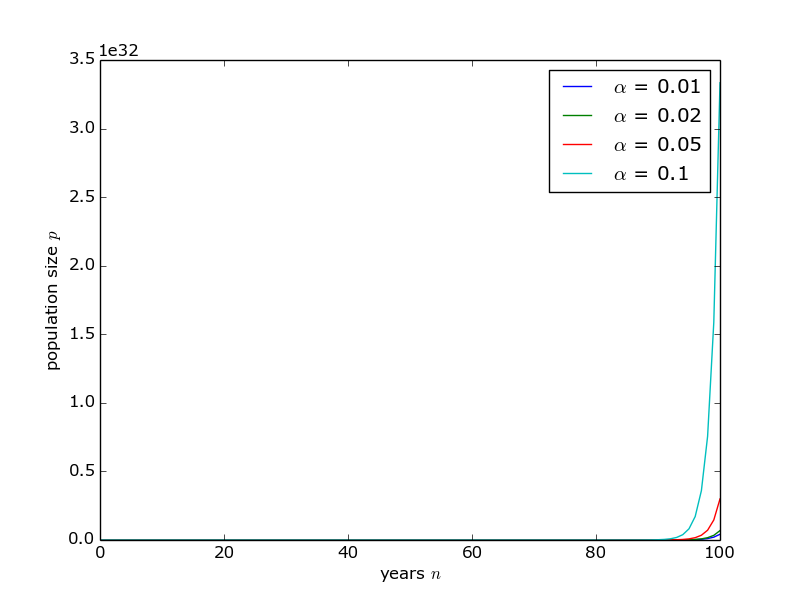
\includegraphics[width=0.7\linewidth]{fig2}
  \caption{Population growth with $p_0 = 2$ and different $\alpha$}
\end{figure}

The population grows more or less fast when $\alpha$ varies. I always keep
$\alpha \le 0.1$ in this figure because if $\alpha$ gets even bigger, the 
population grows really fast and we will not be able to see other curves
with smaller $\alpha$ values.

\vspace{-1em}
\begin{figure}[H]
  \centering
  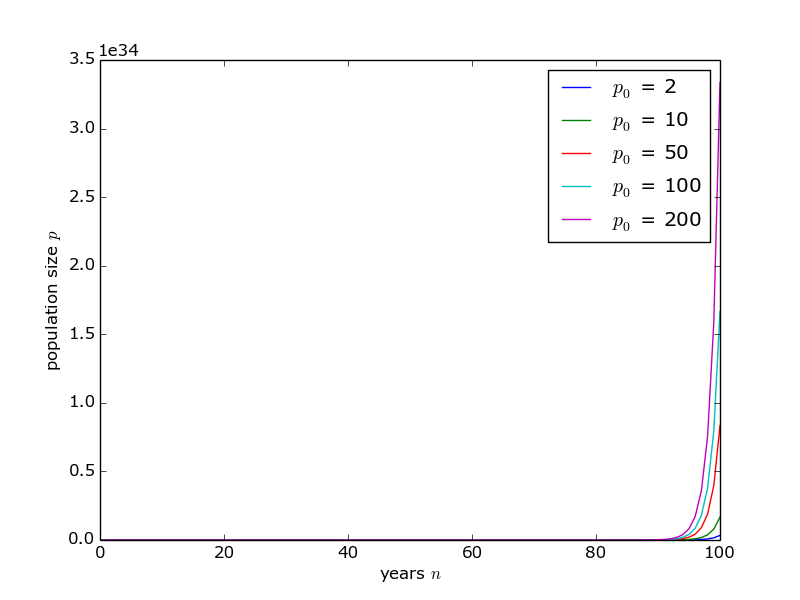
\includegraphics[width=0.7\linewidth]{fig3}
  \caption{Population growth with $\alpha = 0.1$ and different $p_0$}
\end{figure}

In constrast, as shown in the figure above, changing initial population has 
a smaller impact. In fact, the ratio between two different population values
stays constant over time.

\section{Towards a more realistic model}

Nevertheless, the model proposed in the last section is not very satisfying
since the animal population is not meant to grow forever without limitation.
For instance, the problem of resources should be considered, we need to 
modify our model such that $\alpha$ becomes a funcion of $p$, and of course
we want $\alpha$ to decrease when $p$ increases. Let's choose 
$\alpha = 200 - p$.

\vspace{-1em}
\begin{figure}[H]
  \centering
  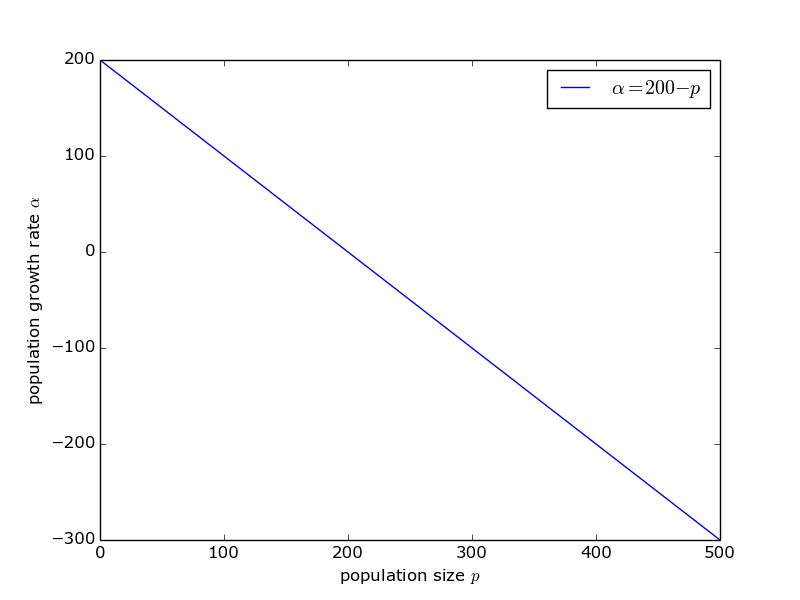
\includegraphics[width=0.7\linewidth]{fig4}
  \caption{Plot of $\alpha = 200 - p$}
\end{figure}

It's quite nice. $\alpha$ is a decreasing function, which means that the 
population will grow more and more slowly as time goes by. It gets even
negative when $p$ is greater than $200$. This prevents the population
from growing too large. However, the real value of $\alpha$ here is too big, 
hence we would rather use $\delta_n = 0.001p_{n-1}(200 - p_{n-1})$ 
(in this case $\alpha = 0.001(200-p_{n-1})$). We can now plot the 
varaiation of the population.

\vspace{-1em}
\begin{figure}[H]
  \centering
  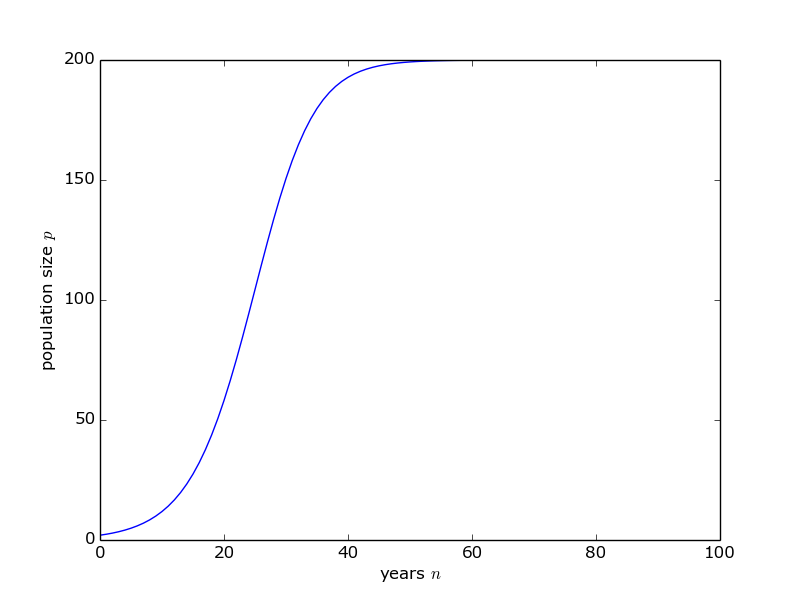
\includegraphics[width=0.7\linewidth]{fig5}
  \caption{Population growth with the law 
           $p_n = p_{n-1} + 0.001p_{n-1}(200 - p_{n-1})$}
\end{figure}

It's closer to the reality this time. We obtain a curve with a sigmoid 
shape. The population grows quite fast at the beginning, but then 
the growth slows down and becomes almost linear, and finally after about
fifty years, the population gets saturated with $p \sim 200$. We can still
try to change different parameters in the equation, like the coefficient
before $200-p$ in $\alpha$.

\vspace{-1em}
\begin{figure}[H]
  \centering
  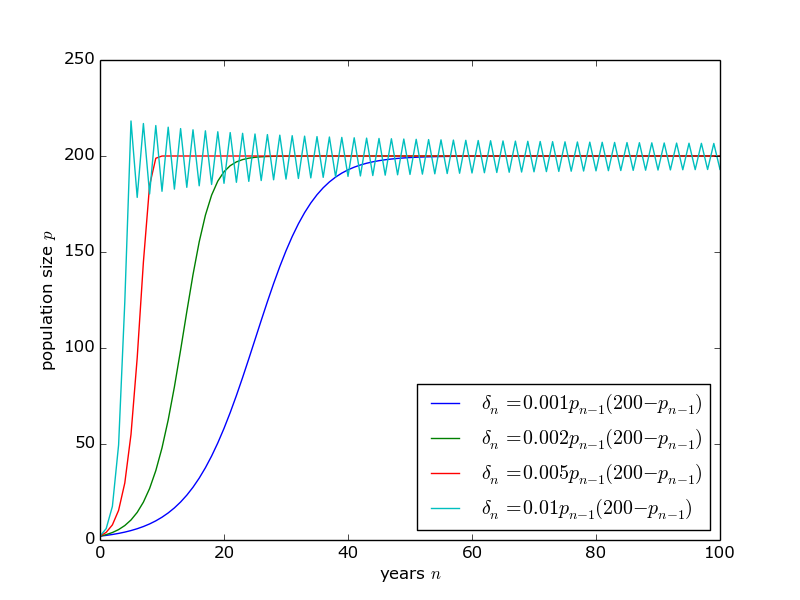
\includegraphics[width=0.7\linewidth]{fig6}
  \caption{Population growth with some different parameters in the law}
\end{figure}

In most of the cases, we see something that is already obeserved: bigger the 
$\alpha$, faster the population grows. Nonetheless, things get more 
interesting when this coefficient becomes bigger ($0.01$ here). An oscillation
behavior appears since the population size can exceed the environment limit
from time to time (but if we keep increasing this parameter, the curve will 
not make sense anymore). At the end of the report, we'd like to see the 
influence of $p_0$ in this model.

\vspace{-1em}
\begin{figure}[H]
  \centering
  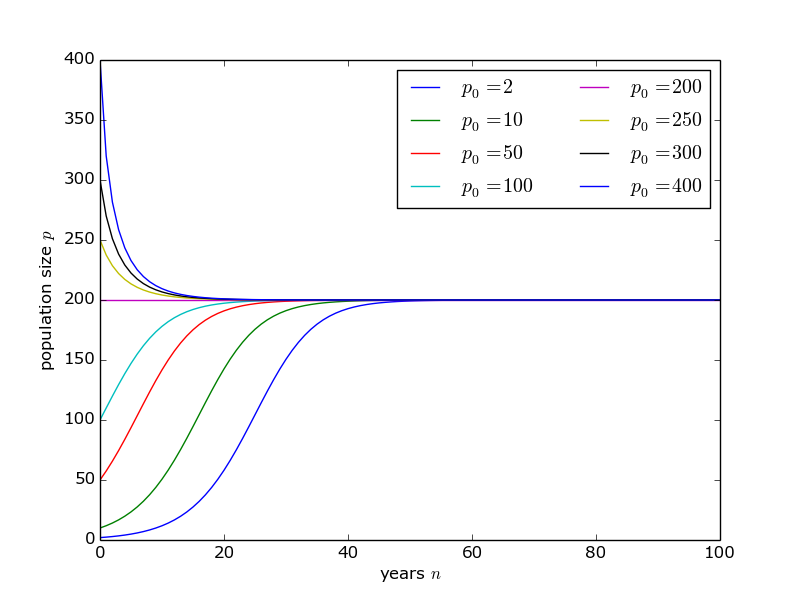
\includegraphics[width=0.7\linewidth]{fig7}
  \caption{Population growth with the same law but different $p_0$}
\end{figure}

It turns out that the result is not that different from what we get from
the first model, but when $p_0$ is larger, the population growth could
become slower from the very beginning (say, we're already in the linear
phase). Furthermore, if $p_0$ is greater than $200$, there aren't 
enough environmental resources for all the individuals, and the
population value will decrease to fit this limitation. A case particular
is when $p_0$ is exactly $200$, the population size will be fixed
from the beginning at $200$.

\section{Conclusion}

In conclusion, we have tried to simulate the animal population growth with
two different models. In the first one, we consider the population growth
rate as a constant and see that the population size can explode very
quickly. Therefore, we decide to take account of resource issues in the
second model. With this extra condition, population saturation is reached
after a period of time and too large population gets penalized.
